In order to tackle the energy efficiency problem of cloud storage systems, we propose
allocating nodes for each user based on the metadata information of that user
and switch the inactive nodes to low energy modes. As described earlier, we assume
a use scenario where a subset of the storage nodes max out the
available bandwidth of the system due to incasting. Therefore, it is not feasible to allocate more
than $M$ nodes to each user both for performance and energy efficiency reasons. Here $M$
represents the number of storage nodes in a subset allocated for a user. Therefore,
the problem we are trying to solve is how to map subsets of the storage nodes to the users.
Since user metadata heterogeneity is well-defined in large-scale cloud systems, we
retrieve user metadata information (i.e. user id, usage pattern) and
allocate subsets of storage nodes to the users using this information.

In this work, we propose three different methods to map cloud storage nodes to the
cloud users, summarized as follows:

\begin{itemize}
\item \textit{Fixed Scheme}: There
are four node allocation techniques in this method: \textit{balancing}, \textit{sequential},
\textit{random} and \textit{grouping} and once one of these techniques is chosen for a
cloud storage system, it remains in effect unless manually changed.
\item \textit{Dynamic Greedy Scheme}: This method
extends the \textit{Fixed Scheme} method by periodically doing dynamic reallocation
among one of the four
allocation techniques (\textit{balancing, sequential, random, grouping}) depending
on their costs. The cost of each technique is calculated based on how important it is
for the cloud storage system to save energy or to balance load.
\item \textit{Correlation-Based Scheme}: This method
monitors user activities and tries to allocate the same subset of storage nodes to the
users who tend to use the cloud storage system concurrently.
\end{itemize}

The energy-aware node allocation methods proposed here are designed to work for a traditional
distributed storage system architecture, but they could also work in a disk array. The
proposed methods not only reduce energy consumption, but also balance load on storage
nodes depending on metrics selected by the cloud administrators.

Before describing each node allocation method in more detail, we first list some of the usage
assumptions in our system and then explain two common
features of the node allocation methods: \textit{inactivity threshold} and \textit{job overlapping}.

We assume that;
\begin{itemize}
\item All storage nodes are initially off and a storage node is started up as soon as a
job arrives.
\item A user uses the same amount of storage space on each of its allocated nodes.
\item Any job run by a user is divided into equal tasks on the nodes allocated for
that user and these tasks are executed concurrently, meaning that they start and
complete simultaneously.
\item If a user is transferred from a subset of the storage nodes to another subset of
the storage nodes, this includes transferring only data. Any jobs that were executed
in the old subset of the storage nodes still belong to those nodes.
\end{itemize}

\paragraph{Inactivity Threshold}
The node allocation methods we are proposing try to save as much energy as possible and
also balance the load on storage nodes depending on metrics selected by the cloud administrators.
If a storage node is not allocated for any user at all, then it will stay in a low-energy mode.
On the other hand, if a storage node is allocated for one or more users, that node will
only switch to a low-energy mode after all jobs using that node are completed.
In an HPC system, the completion time of jobs can be predicted because of job scheduling systems.
Thus, we can decide when to switch a node to a low-energy mode. However, in a cloud storage system,
this predictability is not necessarily always possible, and we need to have a condition to decide when to switch a 
storage node to a low-energy mode. We call this metric the \textit{inactivity threshold}, which
can be defined as \textit{the period of time a node continues to operate at full capacity after the
completion of the most recent storage system job}. This means that, once a node stays inactive for
longer than the inactivity threshold, it can be switched to a
low-energy mode. The \textit{inactivity
threshold}, in this sense, is similar to \textit{break-even time} in previous studies, which ensures
that the energy saved by turning off a node is greater than the energy consumed while switching
that node from active to low-power modes.

In our work, we define the low-energy mode as the state where a node is completely turned off. However,
some modern hard drives have the ability to operate at various
speeds~\cite{Gurumurthi:2003:DDS:871656.859638} thus providing
different levels of energy utilization.
Therefore, in order to conserve energy it is not mandatory to completely turn off a node. Depending on how
much energy saving is demanded by the user, the node allocation techniques can switch nodes into
low-speed operating modes without turning them off. In this work, in order to show the effect of the
node allocation methods better, we assume the worst case and turn off a storage node in low-energy
mode.

If a user is allocated to a node that has been turned off, then that
node needs to start operating at full capacity again. In this case, the user can not immediately access
that storage node, since it will take some time for that node to run at full capacity again. We define the time
it takes to start up a completely turned-off node as the \textit{startup time}. If a storage node has been inactive
between two jobs for longer than the \textit{inactivity threshold}, then the next job on that node
will have to wait for the node to start up.

The \textit{inactivity threshold} and the \textit{startup time} are
important parameters in determining how a real cloud storage
system is going to be affected by the node assignment methods we are proposing.

\paragraph{Job Overlapping}
In a large-scale cloud storage system, each storage node may be used by multiple concurrent users. Our node allocation
methods might allocate a node to multiple users. Therefore, concurrent users can simultaneously
run jobs that use a particular storage node. When two or more jobs overlap on a node, we assume that
node still consumes the same energy per unit
time~\cite{Tsirogiannis:2010:AEE:1807167.1807194}. In other words,
we assume the increased activity due to the multiple jobs will not
increase energy consumption significantly. This is, for the most
part, true because most of the energy is consumed by spinning the
drives not by moving actuators on the drive.

\subsection{Fixed Scheme}
\label{fixed}
In this first scheme, one of the four node allocation techniques described below 
(balancing, sequential, random or grouping) is chosen by the cloud
storage system administrator
and is kept fixed unless manually changed. All techniques have one goal
in common - exploiting user metadata to allocate storage nodes for users. Individually,
each technique performs differently in terms of uniformly allocating storage nodes.
These techniques are each described numerically in Figure~\ref{fixed_examples} with examples.

\begin{figure}[!htbp]
\centering
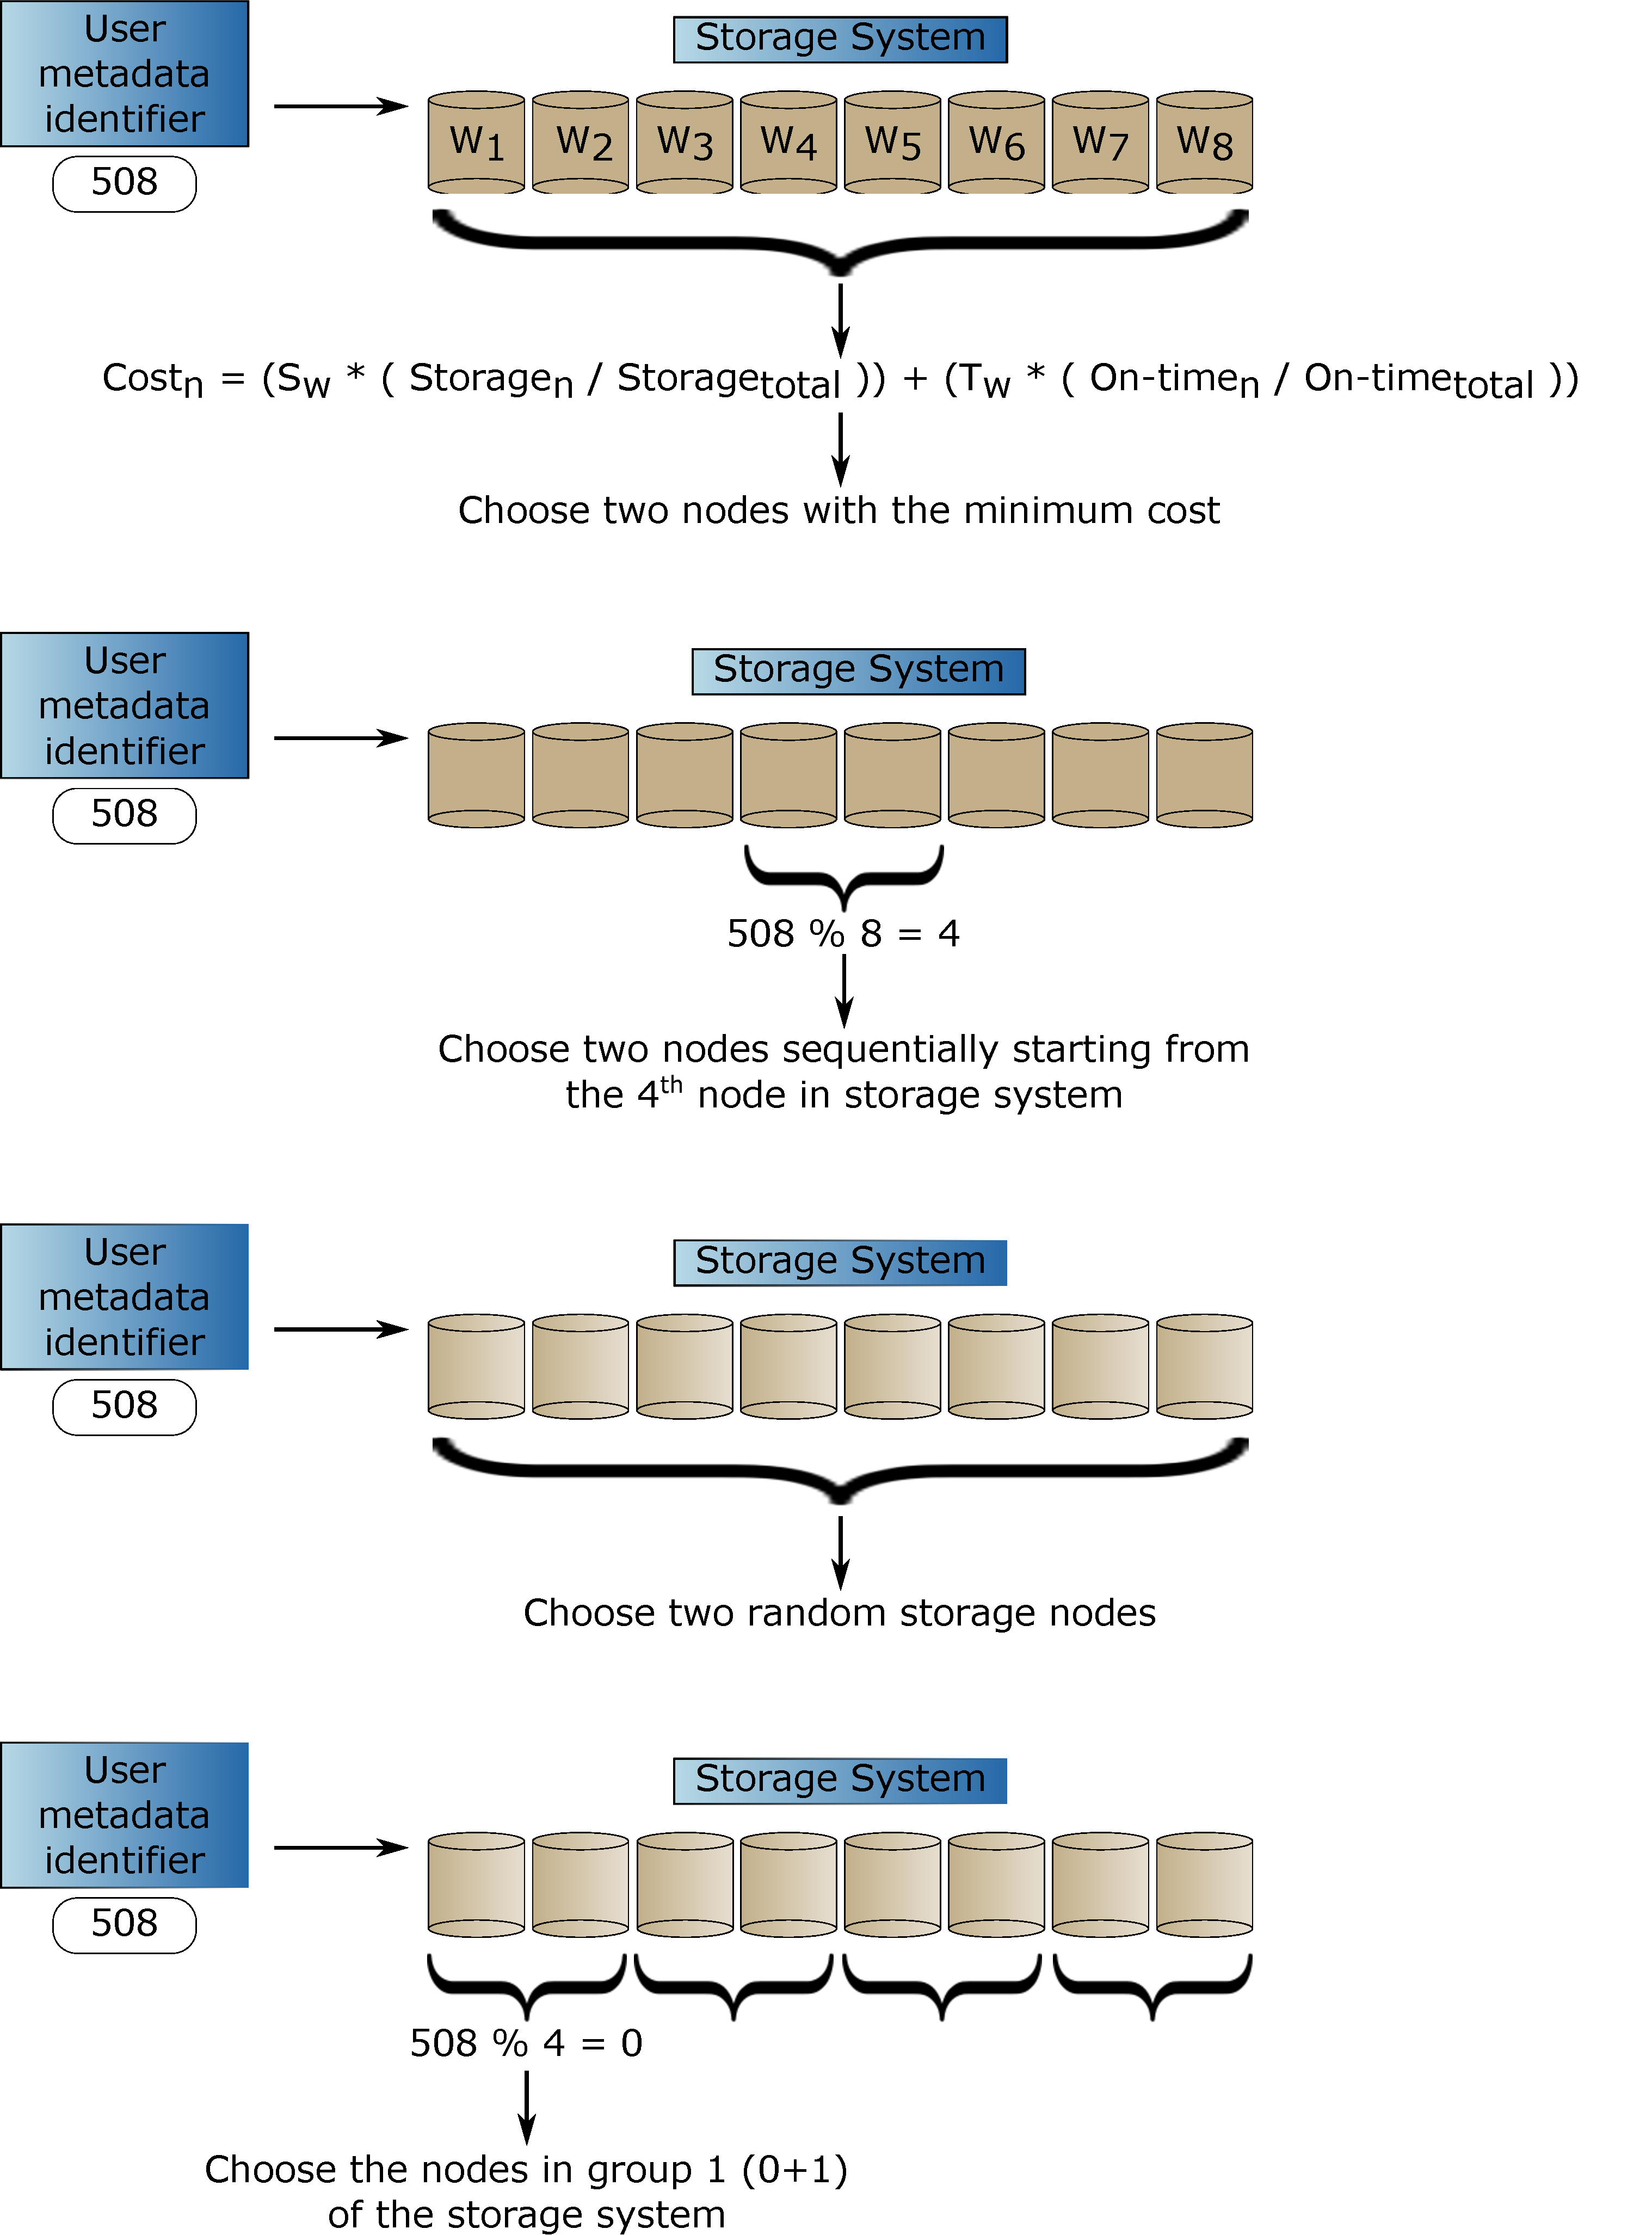
\includegraphics[width=\columnwidth,keepaspectratio]{FIG2.pdf}
\caption{Examples of the node allocation techniques in the Fixed scheme}
\label{fixed_examples}
\end{figure}

\subsubsection{Balancing Technique}
\label{baltechnique}
The primary goal of this technique is to balance the load across the cloud storage nodes. We
define the \textit{load} here in two different ways:

\begin{itemize}
\item The amount of data stored on each node.
\item The total time each node stays on serving user requests.
\end{itemize}

We call balancing the amount of data stored on each node \textit{storage space balancing}.
Similarly, balancing the total time each node stays on is
called \textit{on-time balancing}. These two balancing
techniques ensure that all the nodes in the system are used equally.
Otherwise, the simplest energy saving technique is to simply put all
users and data on the same subset of nodes and permanently turn off
all other nodes. This, however, can cause capacity issues as the
selected nodes may not have enough storage space and also incurs
higher utilization and thus, higher failure rates.
The balancing technique enables system administrators to specify weights for \textit{storage space
balancing} and \textit{on-time balancing} to indicate their importance and allocates
storage nodes for users by adhering to these weights. A \textit{cost} metric is calculated for every
storage node in the system by multiplying storage space and on-time weights with the normalized 
storage space and on-time on that node respectively. In order to normalize storage space and
on-time values, they are divided by the total amount of storage and on-time on all nodes
respectively. In the end, storage nodes with lower costs are preferred by the balancing technique
with the eventual goal of uniformly distributing storage space usage and on-time across storage nodes.
As mentioned previously, we assume the storage space usage of a user is distributed evenly across the
nodes allocated for that user and a job running on multiple nodes concurrently takes the same amount
of time to complete on each node.

Assuming, $N$ is the total number of nodes in the cloud storage system and $M$ is the number
of storage nodes allocated for each user, the balancing technique works as shown in Algorithm~\ref{balapp}.

\begin{algorithm}[!htbp]
\caption{Balancing Technique}
\label{balapp}
\begin{algorithmic}[1]
    \STATE $N \Leftarrow$ Total\ number\ of\ storage\ nodes
    \STATE $M \Leftarrow$ Number\ of\ storage\ nodes\ to\ allocate\ for\ the\ user
    \STATE $ChosenNodes[\ ] \Leftarrow$ Nodes\ that\ will\ be\ allocated\ for\ the\ user
    \STATE $S_{total} \Leftarrow$ Total\ amount\ of\ data\ stored\ on\ all\ nodes
    \STATE $T_{total} \Leftarrow$ Total\ duration\ of\ time\ all\ nodes\ stayed\ on
    \STATE $S_i \Leftarrow$ Amount\ of\ data\ stored\ on\ node\ $i$
    \STATE $T_i \Leftarrow$ Duration\ of\ time\ node\ $i$ stayed\ on
    \STATE $S_W \Leftarrow$ Importance\ of\ balancing\ storage\ space
    \STATE $T_W \Leftarrow$ Importance\ of\ balancing\ time
    \STATE $Costs[\ ] \Leftarrow$ Costs\ of\ nodes\ $i$
    \FOR{$i=1$ to $N$}
        \STATE $Costs[i] \Leftarrow (S_W * (S_i/S_{total}) + (T_W * (T_i/T_{total}))$
    \ENDFOR
    \FOR{$i=1$ to $M$}
        \STATE $ChosenNodes[i] \Leftarrow min(Costs[\ ])$
        \STATE Remove $min(Costs[\ ])$ from $Costs[\ ]$
    \ENDFOR
\end{algorithmic}
\end{algorithm}

The storage space and on-time weights should add up to 1. As an example, if it is equally important
to balance storage space and on-time for a system
administrator, then $S_W=T_W=0.5$. However, if it is more important to
balance storage space, then $S_W=1$ and $T_W=0$.

\subsubsection{Sequential Technique}
\label{seqtechnique}
The sequential technique use an approach similar to consistent hashing~\cite{Karger:1997:CHR:258533.258660}.
%Assuming $N$ is the total number of nodes in the cloud storage system and $M$ is the number
%of storage nodes allocated for each user;
The approach starts by calculating an $Offset$
value for a given user
with metadata information represented by $I$. As described earlier, 
this metadata information can be a user id or user home directory, basically any metadata information
that can be hashed to an integer.

Given this hash value, one can then sequentially allocate storage nodes for the user starting from
the storage node with an identifier equal to $Offset$.
%Considering that nodes in distributed storage
%systems are usually given numbers such as \textit{(001,002,...)} to indicate their order, this is a
%reasonable approach. As we mentioned earlier, $M$ is the number of storage nodes allocated for
%each user.
The $M$ nodes following the storage node with identifier equal to $Offset$ are
allocated for a user in the sequential technique.
%Assuming, $N$ is the total number of nodes in the
%cloud storage system and $M$ is the number of storage nodes allocated
%for each user
A summary of the sequential
technique is shown in Algorithm~\ref{seqapp}.

\begin{algorithm}[!htbp]
\caption{Sequential Technique}
\label{seqapp}
\begin{algorithmic}[1]
    \STATE $N \Leftarrow$ Total\ number\ of\ storage\ nodes
    \STATE $M \Leftarrow$ Number\ of\ storage\ nodes\ to\ allocate\ for\ the\ user
    \STATE $I \Leftarrow$ Metadata\ information\ of\ the\ user
    \STATE $Offset \Leftarrow$ Identifier\ of\ storage\ node\ from\ which\ allocation\ will\ start
    \STATE $ChosenNodes[\ ] \Leftarrow$ Nodes\ that\ will\ be\ allocated\ for\ the\ user
    \STATE $Offset \Leftarrow I\ mod\ N$
    \FOR{$i=1$ to $M$}
        \STATE $ChosenNodes[i] \Leftarrow (Offset\ +\ i)\ mod\ M$
    \ENDFOR
\end{algorithmic}
\end{algorithm}

Note that in Algorithm~\ref{seqapp} on line 6, we are taking the modulus of node identifiers in order to
make sure they are smaller than the total number of nodes in the cloud
storage system, $N$.
%This is because the starting offset calculated in the the sequential technique may be close to the last
%storage node in the system, such that when $M$ storage nodes are sequentially assigned to a user,
%we may run out of storage nodes in the system. In this case the node allocation continues with the
%first storage node.

\subsubsection{Random Technique}
The random technique uses a random number generator that chooses an identifier of a storage node
in the system. The random number generator is called $M$ times to generate $M$ different identifiers.
These identifiers represent the storage nodes that will be allocated for a user. The
random function is seeded with the user's arrival time to the storage system, giving enough
randomness. Still, if it produces an identifier twice, it is called until all $M$ identifiers
in the subset are distinct. Assuming, $N$ is the total number of nodes in the
cloud storage system and $M$ is the number of storage nodes allocated for each user, the random
technique works as shown in Algorithm~\ref{randapp}.

\begin{algorithm}[!htbp]
\caption{Random Technique}
\label{randapp}
\begin{algorithmic}[1]
    \STATE $N \Leftarrow Total\ number\ of\ storage\ nodes$
    \STATE $M \Leftarrow Number\ of\ storage\ nodes\ to\ allocate\ for\ the\ user$
    \STATE $ChosenNodes[\ ] \Leftarrow Nodes\ that\ will\ be\ allocated\ for\ the\ user$
    \FOR{$i=1$ to $M$}
        \WHILE{$j\ \in ChosenNodes[\ ]$}
            \STATE $j \Leftarrow rand()$
        \ENDWHILE
        \STATE $ChosenNodes[i] \Leftarrow j$
    \ENDFOR
\end{algorithmic}
\end{algorithm}

\subsubsection{Grouping Technique}
The grouping technique is similar to the sequential technique described in Section~\ref{seqtechnique}.
Compared to the sequential technique, the grouping technique has fewer starting points(\textit{offset})
to choose. %Assuming, $N$ is the total number of nodes in the cloud storage system and $M$ is the
%number of storage nodes allocated for each user;
First, node groups of size $M$ are
created where $M$ sequential storage nodes together form a
group. Here, for ease of explanation, we 
assume that total number of nodes, $N$, is a multiple of the number of storage nodes allocated
for each user, $M$. For systems where this is not true, groups may be overlapped. At this point,
we assume $G\ =\ N\ /\ M$ groups are created in the systems, where $G$ denotes the number of groups created. 
Then, similar to the sequential technique, a group is chosen using the given user's metadata information
represented by $I$ and the storage nodes in that group are allocated for that user. As described
earlier, this metadata information can be user id or user home directory, basically any metadata
information that can be hashed to an integer. The grouping technique works as shown in
Algorithm~\ref{groupapp}.

\begin{algorithm}[!htbp]
\caption{Grouping Technique}
\label{groupapp}
\begin{algorithmic}[1]
    \STATE $N \Leftarrow$ Total\ number\ of\ storage\ nodes
    \STATE $M \Leftarrow$ Number\ of\ storage\ nodes\ to\ allocate\ for\ the\ user
    \STATE $G \Leftarrow$ Number\ of\ storage\ node\ groups
    \STATE $I \Leftarrow$ Metadata\ information\ of\ the\ user $\Leftarrow N\ /\ M$
    \STATE $Offset \Leftarrow$ Identifier\ of\ node\ group\ which\ will\ be\ allocated\ for\ the\ user
    \STATE $ChosenNodes[\ ] \Leftarrow$ Nodes\ that\ will\ be\ allocated\ for\ the\ user
    \STATE $Offset \Leftarrow I\ mod\ G$
    \FOR{$i=1$ to $M$}
        \STATE $ChosenNodes[i] \Leftarrow (G\ *\ M)\ +\ i$
    \ENDFOR
\end{algorithmic}
\end{algorithm}

\subsection{Dynamic Greedy Scheme}
\label{greedy}
In this method, one of the four node allocation techniques described in Section~\ref{fixed} (balancing,
sequential, random or grouping) is initially chosen by the cloud system and that technique is re-evaluated
against other techniques at certain times (called as \textit{evaluation points}) over a recent period (called
as \textit{control period}), in terms of energy efficiency and/or load balancing. If there is a better
technique in terms of energy efficiency and/or load balancing and if the cost of switching to that technique
is less than the energy to be saved by switching to that technique, then the current technique is changed.
The \textit{Dynamic Greedy Scheme} is described in Algorithm~\ref{greedyapp}.

In this scheme, we use coefficient or variation (CV) amongst the nodes as a proxy for storage space
and on-time balancing.
In other words, a high CV indicates that the storage
space or on-time is not well balanced.
The \textit{Dynamic Greedy Scheme} first multiplies the normalized CVs of storage space
and on-time ($Svar$ and $Tvar$ in Algorithm~\ref{greedyapp}) with their corresponding importance
weights ($S_W$ and $T_W$). In order to normalize the CVs of storage space and on-time, they are
divided by the maximum possible CV of storage space ($MaxSvar$) and on-time
($MaxTvar$) respectively. The maximum CV of storage space and on-time occurs when all requests
are served by a single storage node and this sets an upper limit on the CV value. Then the multiplication
of the normalized energy cost ($ECost$) with the energy consumption weight ($E_W$) is added to this product. Energy
cost includes both the energy consumption due to running jobs according to a technique ($JobCost$) and the energy
consumption due to transferring user data while switching to that technique ($TrnCost$). Energy cost ($ECost$) is
divided by the sum of maximum cost of jobs ($MaxJobCost$) and the maximum cost of data transfers ($MaxTrnCost$) over the 
\textit{control period}. Maximum job cost ($MaxJobCost$) occurs when all nodes are left on all the time. Maximum data
transfer cost ($MaxTrnCost$) occurs when all data existing in the storage system is moved.

A cloud system administrator can specify different values for storage space, on-time and energy consumption
weights ($S_W$, $T_W$ and $E_W$). This enables a fine-grained control over load-balancing and energy consumption
in a cloud storage system. As discussed in Section~\ref{baltechnique}, the storage space
and on-time weights add up to 1. The energy consumption weight is independent of the other two, meaning that,
a cloud system administrator might prefer to save energy regardless of load-balancing decisions. 

\begin{algorithm}[!htbp]
\caption{Dynamic Greedy Scheme}
\label{greedyapp}
\begin{algorithmic}[1]
    \STATE $P \Leftarrow$ Number\ of\ available\ node\ allocation\ techniques
    \STATE $S_W \Leftarrow$ Importance\ of\ balancing\ storage\ space
    \STATE $T_W \Leftarrow$ Importance\ of\ balancing\ time
    \STATE $E_W \Leftarrow$ Importance\ of\ reducing\ energy\ consumption
    \STATE $Svar_i \Leftarrow$ CV\ of\ storage\ space\ across\ all\ nodes\ for\ technique\ $i$
    \STATE $MaxSvar \Leftarrow$ Maximum\ possible\ CV\ of\ storage\ space\ across\ all\ nodes
    \STATE $Tvar_i \Leftarrow$ CV\ of\ on-time\ across\ all\ nodes\ for\ technique\ $i$
    \STATE $MaxTvar \Leftarrow$ Maximum\ possible\ CV\ of\ on-time\ across\ all\ nodes
    \STATE $JobCost_i \Leftarrow$ Cost\ of\ all\ jobs\ in\ the\ control\ period\ for\ technique\ $i$
    \STATE $TrnCost_i \Leftarrow$ Cost\ of\ data\ transfers\ while\ switching\ to\ technique\ $i$
    \STATE $ECost_i \Leftarrow JobCost_i + TrnCost_i$
    \STATE $MaxJobCost \Leftarrow$ Maximum\ cost\ of\ all\ jobs\ \ over\ the\ control\ period
    \STATE $MaxTrnCost \Leftarrow$ Maximum\ cost\ of\ all\ data\ transfers\ over\ the\ control\ period
    \STATE $TotalCost_i \Leftarrow$ Total\ cost\ of\ technique\ i\ at\ an\ evaluation\ point
    \STATE $MinCost \Leftarrow$ Minimum\ technique\ cost\ observed\ so\ far
    \STATE $NewTechq \Leftarrow$ Technique\ that\ will\ be\ in\ affect\ after\ the\ evaluation

    \STATE $MinCost \Leftarrow 0$
    \STATE $NewTechq \Leftarrow 0$
    \FOR{$i=1$ to $P$}
        \STATE $TotalCost_i \Leftarrow (S_W\ *\ (Svar_i\ /\ MaxSvar))\ +\ (T_W\ *\ (Tvar_i\ /\ MaxTvar))\ +\ (E_W\ *\ (ECost_i\ /\ (MaxJobCost\ +\ MaxTrnCost)))$
        \IF{$MinCost == 0\ \OR\ TotalCost_i < MinCost$}
            \STATE $NewTechq \Leftarrow i$
            \STATE $MinCost \Leftarrow TotalCost_i$
        \ENDIF
    \ENDFOR
\end{algorithmic}
\end{algorithm}

The parameters of a technique evaluation can be summarized as follows:
\begin{itemize}
\item \textbf{The frequency of the technique evaluations}: The system administrator might decide to
evaluate the current node allocation technique of the system against other techniques every couple of
hours, days etc.
\item \textbf{Jobs to evaluate}: Ideally, all jobs that have been submitted to the storage system so far
should be evaluated to compare node allocation techniques with each other. However, this might prove to be costly due
to the potentially large number of jobs submitted before an \textit{evaluation point}. Therefore, the system
administrator specifies a \textit{control period} that specifies the
time period from which the jobs are used to evaluate the node
allocation techniques at every \textit{evaluation point}.
The \textit{control period} again can be couple of hours, days etc., but it has to be less than the frequency of
technique evaluations to make sure that evaluations at different moments do not interfere with each other.
\item \textbf{What is important while comparing node allocation techniques}: Cloud system administrators might be
concerned with different aspects of the cloud storage system. As an example, different values can be specified for
storage space, on-time and energy consumption weights ($S_W$, $T_W$ and $E_W$)
\end{itemize}

Figure~\ref{greedy_examples} gives a numerical example of
the \textit{Dynamic Greedy Scheme}.
A cloud storage system administrator can evaluate node allocation techniques (balancing, sequential, random,
grouping) every 4 days by looking at the jobs submitted in the last 6 hours and by trying to save as much energy
as possible while trying to balance the storage space only across the nodes. Our work in this sense is similar
to the studies that try to predict idle periods or node reservation lengths~\cite{4724317, Riska:2010:FRE:1710115.1710124},
but the way we are predicting the future is much simpler compared to those studies. We simply look at the jobs
going back to a specified duration of time (a.k.a. \textit{control period}). However, existing studies instrument
and monitor cloud systems with complex mechanisms to collect feedback and hints.

\begin{figure}[!htbp]
\centering
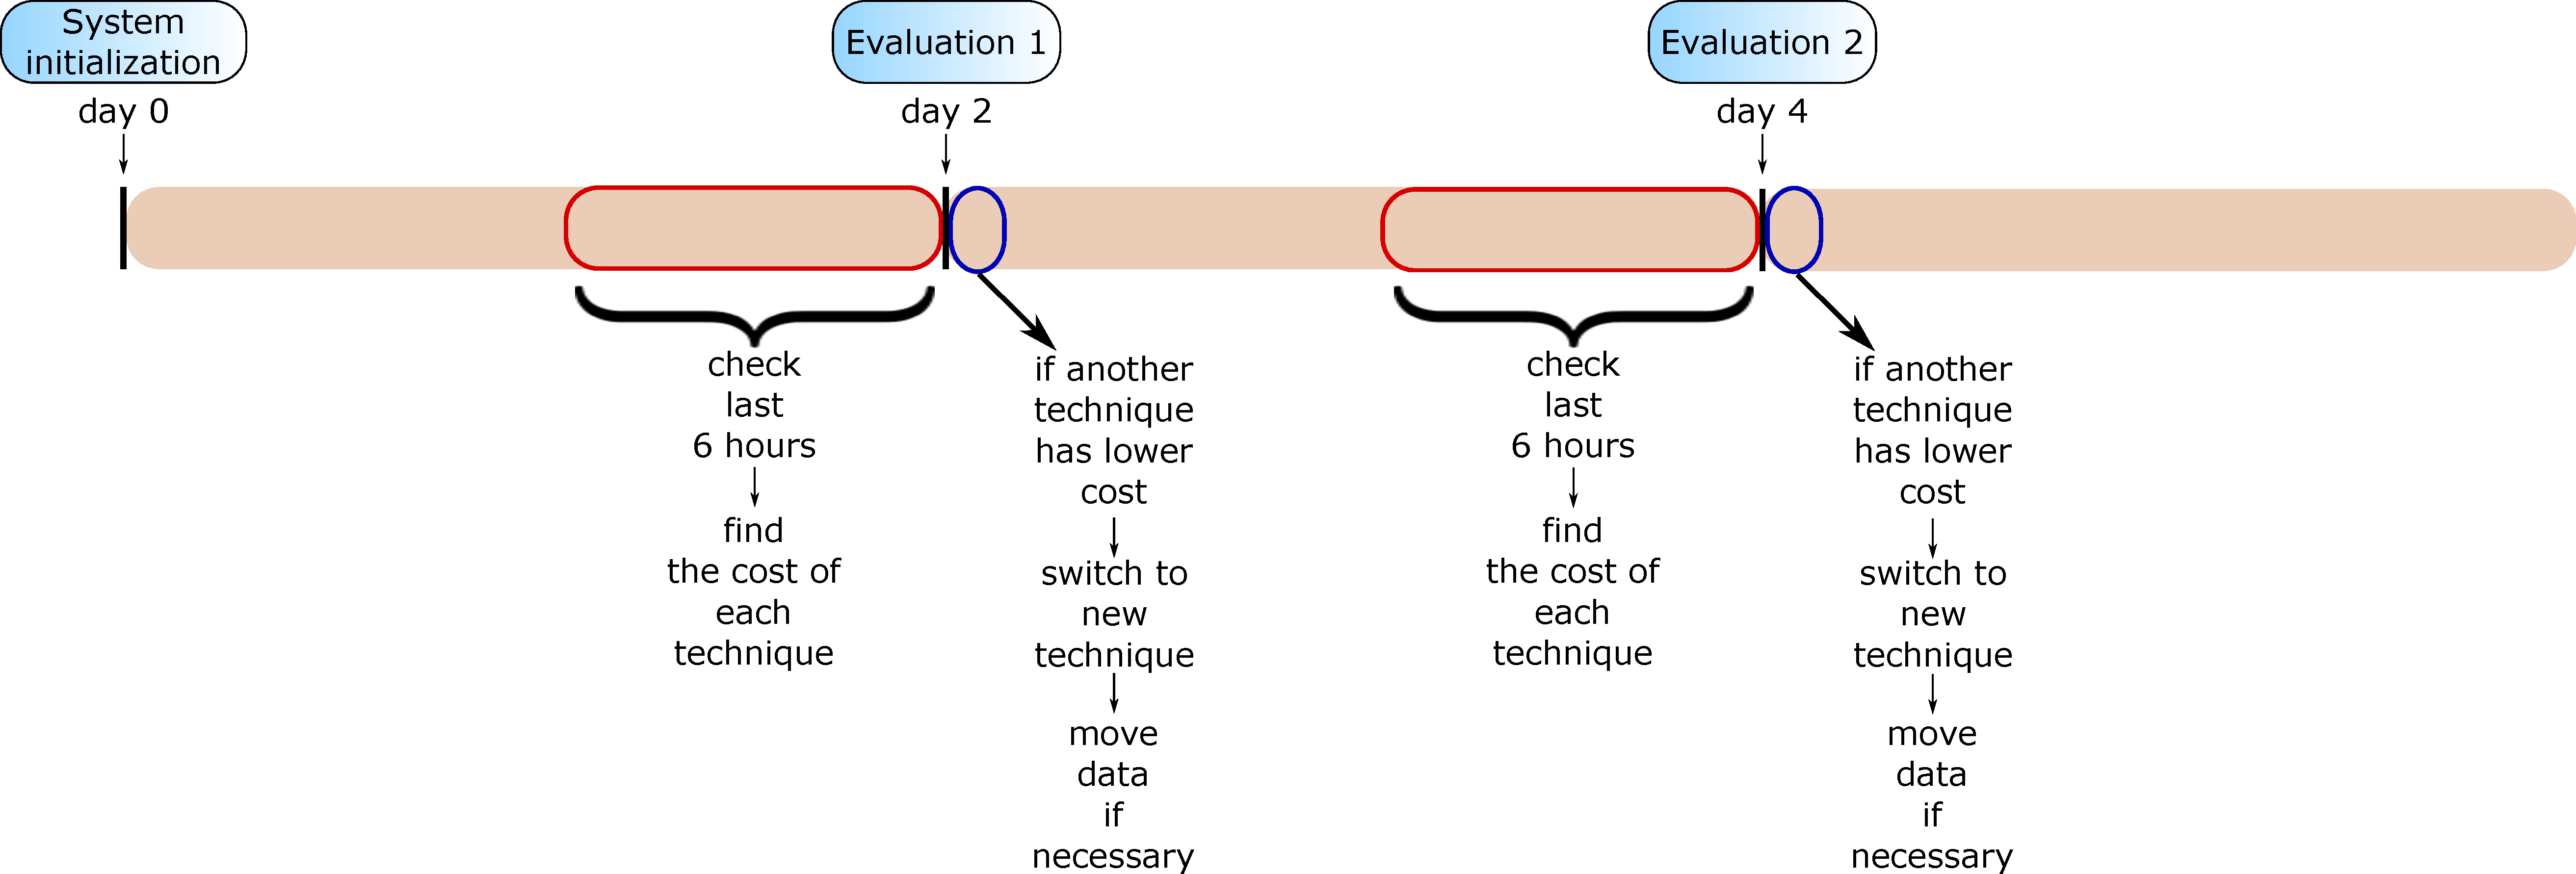
\includegraphics[width=\columnwidth,keepaspectratio]{FIG3.pdf}
\caption{Example of the Dynamic Greedy scheme (evaluations done at every 2 days, last 6 hours are checked only)}
\label{greedy_examples}
\end{figure}

\subsection{Correlation-Based Scheme}
\label{correlation}
This scheme is similar to the \textit{Dynamic Greedy Scheme} described in Section~\ref{greedy}, in the sense that
the node allocations are evaluated periodically at \textit{evaluation points} over a recent period (called
as \textit{control period}). However, rather than switching between node allocation
techniques (balancing, sequential, random, grouping) at \textit{evaluation points}, \textit{Correlation-Based Scheme}
starts with one of these techniques (can be chosen randomly) and keeps using that technique unless it is manually
changed. \textit{Correlation-Based Scheme} monitors user activities over the recent \textit{control period} and
allocates the same subset of cloud storage nodes to the users who tend to use the system in similar fashion.
Here, we define the similarity between users as concurrent usage of the cloud storage system, meaning that if
two or more users use the cloud storage system for longer than a threshold (called as \textit{similarity threshold}
in Algorithm~\ref{corrapp}) cumulatively, then same subset of storage nodes are allocated for them. We need
user access times as the metadata information to find concurrent user accesses, but other metadata (i.e.
number of accesses, amount of data stored) can be used as well to assess similarity between users.
Figure~\ref{correlation_examples} gives a numerical example of the \textit{Correlation-Based Scheme}.

\begin{figure}[!htbp]
\centering
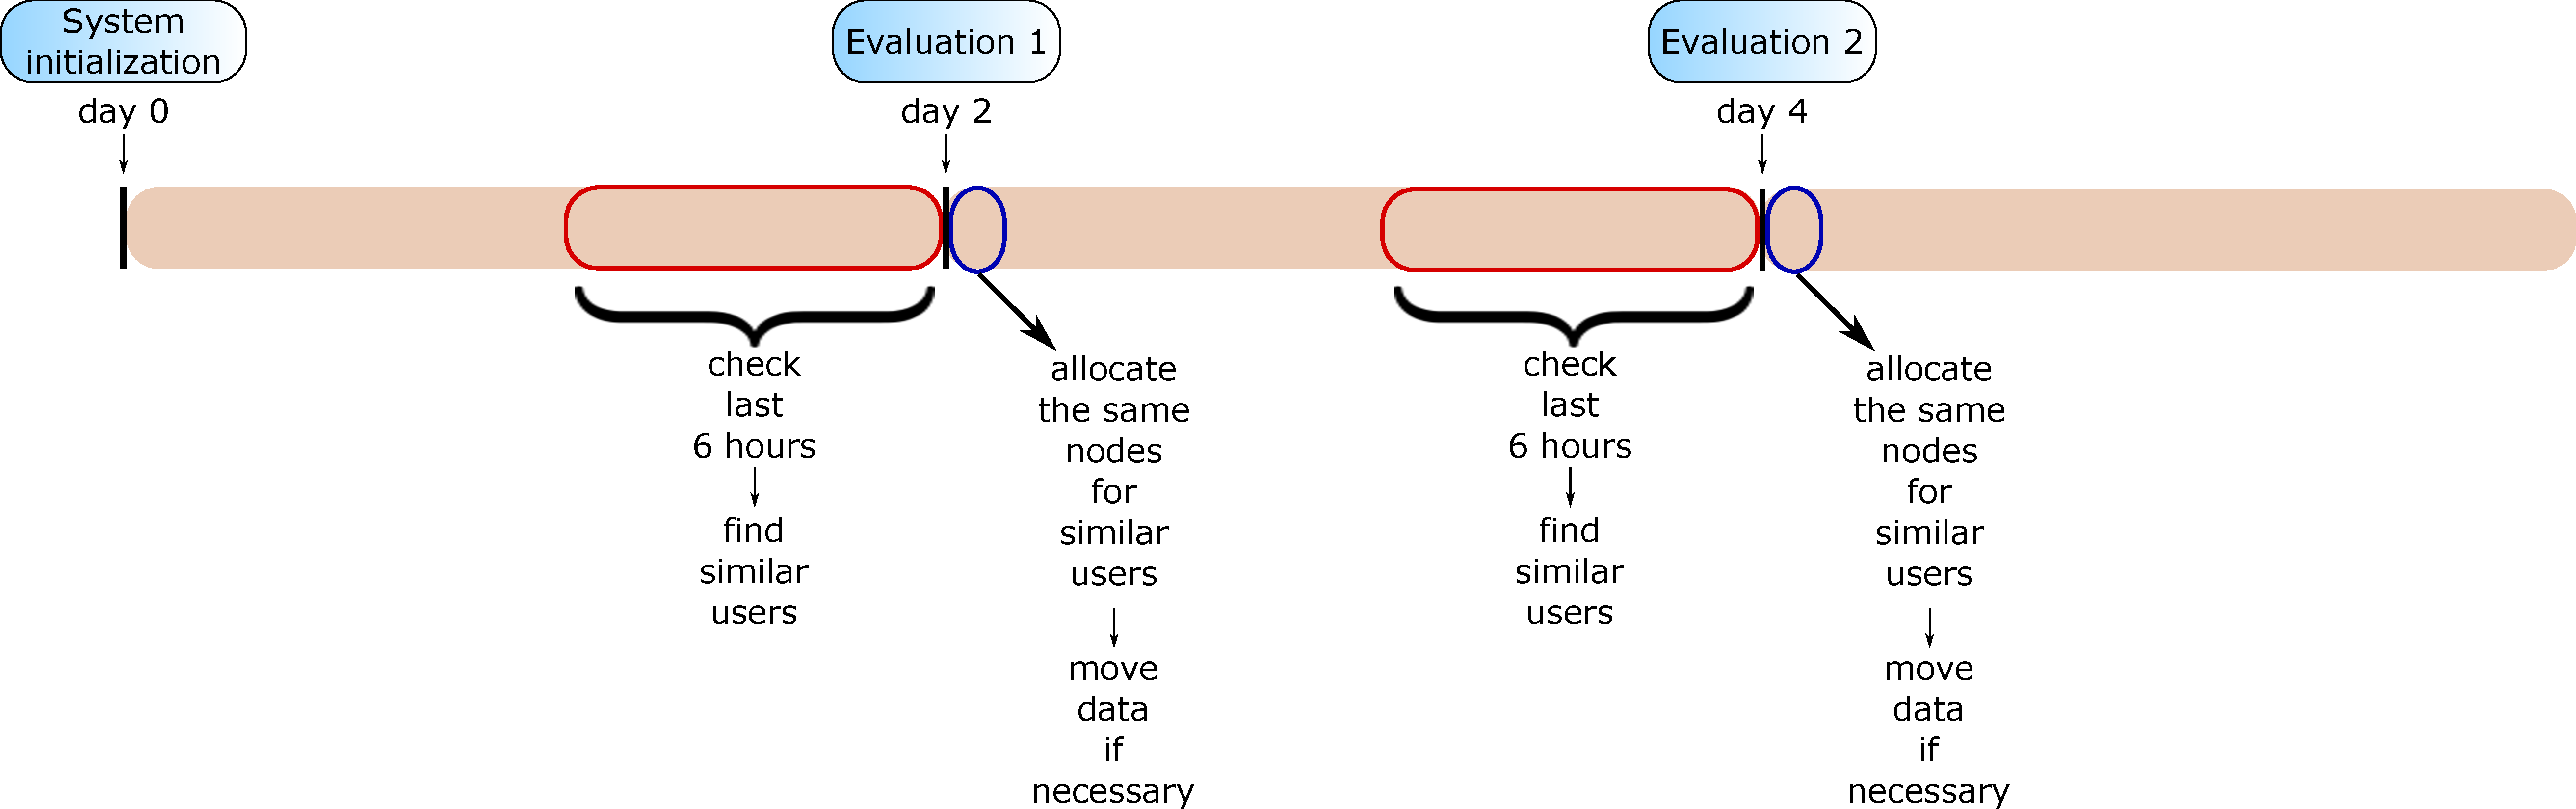
\includegraphics[width=\columnwidth,keepaspectratio]{FIG4.pdf}
\caption{Example of the Correlation-Based scheme (evaluations done at every 2 days, last 6 hours are checked only)}
\label{correlation_examples}
\end{figure}

The \textit{similarity threshold} sets a lower limit to define the concurrent usage of the storage system. As
an example, if the \textit{similarity threshold} is 4 hours, two or more users using the cloud storage systems
for more than 4 hours cumulatively are going to be assigned the same storage nodes. Here, it is important to point
out that the \textit{Correlation-Based Scheme} evaluates concurrent user activities cumulatively, meaning that, if
two or more users access the system concurrently for 3 hours in the morning and then for 1 hour in the afternoon,
those users will be considered as using the storage system in a similar fashion and they will be assigned the
same subset of cloud storage nodes. The \textit{Correlation-Based Scheme} is described in
Algorithm~\ref{corrapp}. 

\begin{algorithm}[!htbp]
\caption{Correlation-Based Scheme}
\label{corrapp}
\begin{algorithmic}[1]
    \STATE $T_{similar} \Leftarrow Similarity\ threshold$
    \STATE $R \Leftarrow Number\ of\ similarities\ between\ users\ in\ the\ most\ recent\ control\ period$
    \STATE $Similarities[\ ] \Leftarrow Array\ storing\ duration\ of\ user\ similarities$
    \FOR{$i=1$ to $R$}
        \IF{$Similarities[i] > T_{similar}$}
            \STATE Allocate the same storage nodes for users in this similarity
        \ENDIF
    \ENDFOR
\end{algorithmic}
\end{algorithm}

